\documentclass[conference]{IEEEtran}
\IEEEoverridecommandlockouts
% The preceding line is only needed to identify funding in the first footnote. If that is unneeded, please comment it out.
%Template version as of 6/27/2024

\usepackage{cite}
\usepackage{amsmath,amssymb,amsfonts}
\usepackage{algorithmic}
\usepackage{graphicx}
\usepackage{textcomp}
\usepackage{xcolor}
\usepackage{tabularx}
\usepackage{array}
\graphicspath{{figs/}{inputs/}{outputs/}}
\def\BibTeX{{\rm B\kern-.05em{\sc i\kern-.025em b}\kern-.08em
    T\kern-.1667em\lower.7ex\hbox{E}\kern-.125emX}}
\begin{document}

\title{Construcción de Imágenes Panorámicas mediante Homografías: \\ Detección de Características, DLT y RANSAC}

\author{
\IEEEauthorblockN{Vocos Conesa, Tomás}
\IEEEauthorblockA{\textit{Ingeniería en Inteligencia Artificial} \\
\textit{Universidad de San Andrés}\\
Buenos Aires, Argentina \\
tvocosconesa@udesa.edu.ar}
\and
\IEEEauthorblockN{De Hieronymis, Martín Ariel}
\IEEEauthorblockA{\textit{Ingeniería en Inteligencia Artificial} \\
\textit{Universidad de San Andrés}\\
Buenos Aires, Argentina \\
mdehieronymis@udesa.edu.ar}
\and
\IEEEauthorblockN{Larisson, Zoe}
\IEEEauthorblockA{\textit{Ingeniería en Inteligencia Artificial} \\
\textit{Universidad de San Andrés}\\
Buenos Aires, Argentina \\
zlarisson@udesa.edu.ar}
}

\maketitle

\begin{abstract}
Se implementa un pipeline completo de construcción de imágenes panorámicas a partir de conjuntos de tres imágenes con solapamiento parcial. El método detecta características locales mediante SIFT, las redistribuye espacialmente con Supresión de No Máxima Adaptativa (A-NMS), establece correspondencias con verificación cruzada y el test de razón de Lowe, estima homografías tanto de forma manual (DLT sobre 4 correspondencias) como robusta (RANSAC), calcula el tamaño óptimo del lienzo final y funde las imágenes proyectadas mediante una máscara de distancia. El método se evaluó sobre el conjunto provisto \textit{cuadro} y sobre un conjunto propio de tres fotografías del campus de la universidad.
\end{abstract}

\section{Introducción}

Una imagen digital es el resultado de proyectar una escena tridimensional sobre un plano a través de un modelo de cámara \textit{pinhole}. Dos fotografías de una misma escena, tomadas con la misma cámara desde distintas posiciones, están relacionadas por una transformación proyectiva lineal de $3\times3$ (\emph{homografía}, $H$, con 8 grados de libertad) que mapea puntos homogéneos $\mathbf{x}$ de una imagen a puntos $\mathbf{x}'$ de la otra ($\mathbf{x}' \sim H\mathbf{x}$) \textbf{si y solo si} se cumple alguna de las siguientes dos hipótesis geométricas:

\begin{enumerate}
    \item La escena observada es (aproximadamente) \textbf{plana}, o
    \item La cámara sufrió únicamente una \textbf{rotación pura} alrededor de su centro óptico entre una toma y la otra, sin traslación.
\end{enumerate}

Bajo cualquiera de estas dos hipótesis, la relación entre imágenes no depende de la profundidad de la escena, por lo que una única matriz $H$ alcanza para alinear todos los puntos. Cuando ninguna de las dos hipótesis se cumple exactamente --es decir, cuando la cámara se traslada y la escena tiene profundidad variable-- aparece \textbf{paralaje}: objetos a distinta distancia de la cámara se desplazan de forma distinta entre las dos vistas, y ninguna homografía única puede alinearlos a todos simultáneamente. El síntoma visible de esto es \emph{ghosting} (objetos duplicados o desalineados) en la zona de solapamiento, particularmente en los objetos más cercanos a la cámara.

\textbf{Análisis de los conjuntos utilizados:} El conjunto \textit{cuadro} (Fig.~\ref{fig:dataset_cuadro}) corresponde a un cuadro apoyado sobre una mesa, fotografiado desde tres posiciones cercanas. La escena es aproximadamente plana (el cuadro domina el campo visual), por lo que la hipótesis (1) se cumple razonablemente bien; el principal apartamiento proviene de que las tomas no son una rotación pura sino que incluyen un leve desplazamiento lateral de la cámara sobre la mesa, lo que introduce paralaje leve respecto del borde de la mesa y del piso, visibles como fondo no plano. El conjunto propio (fotos del campus, Fig.~\ref{fig:panorama_propio}) es lo opuesto: la escena \emph{no} es plana (edificio, césped y árboles a distintas profundidades), pero las tres fotos fueron tomadas girando la cámara sobre un mismo punto aproximado, por lo que se aproxima mejor a la hipótesis (2). El paralaje residual se manifiesta principalmente en los árboles del primer plano, que son los objetos más cercanos a la cámara.

\begin{figure}[htbp]
\centering
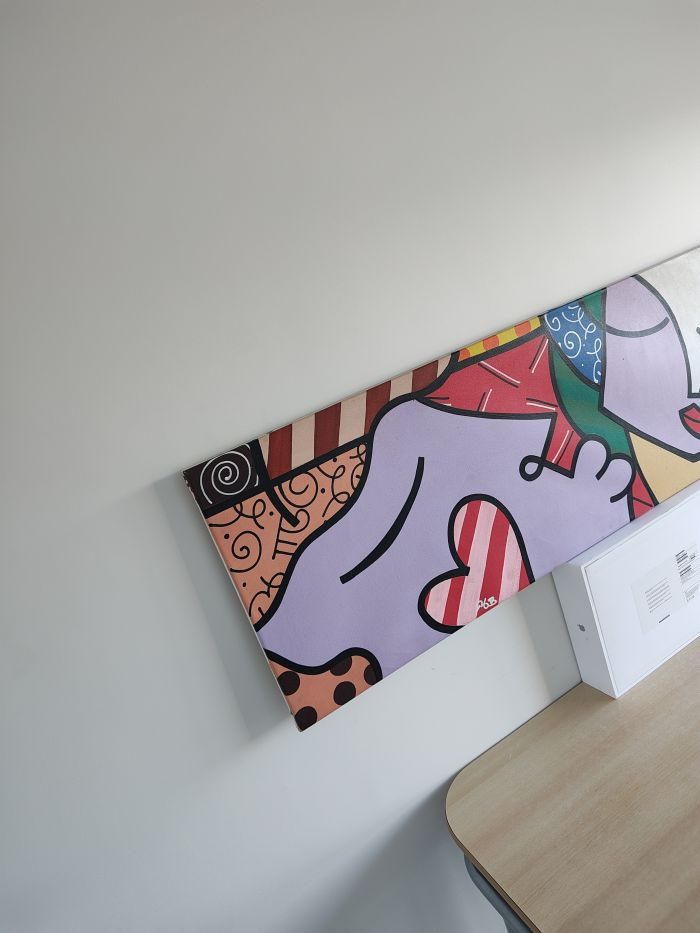
\includegraphics[width=0.32\linewidth]{cuadro_0_thumb.jpg}
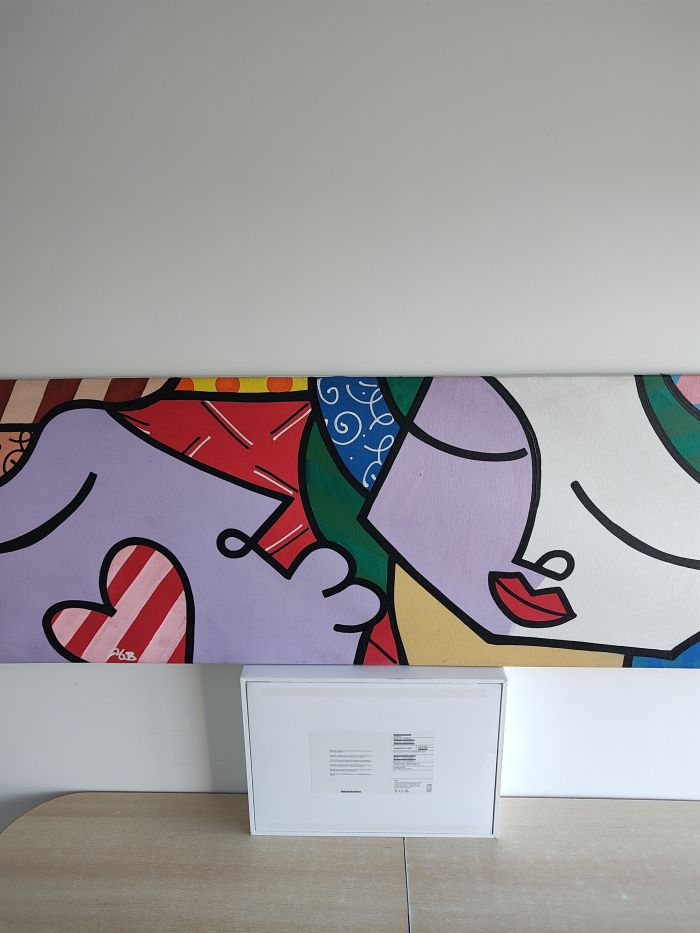
\includegraphics[width=0.32\linewidth]{cuadro_1_thumb.jpg}
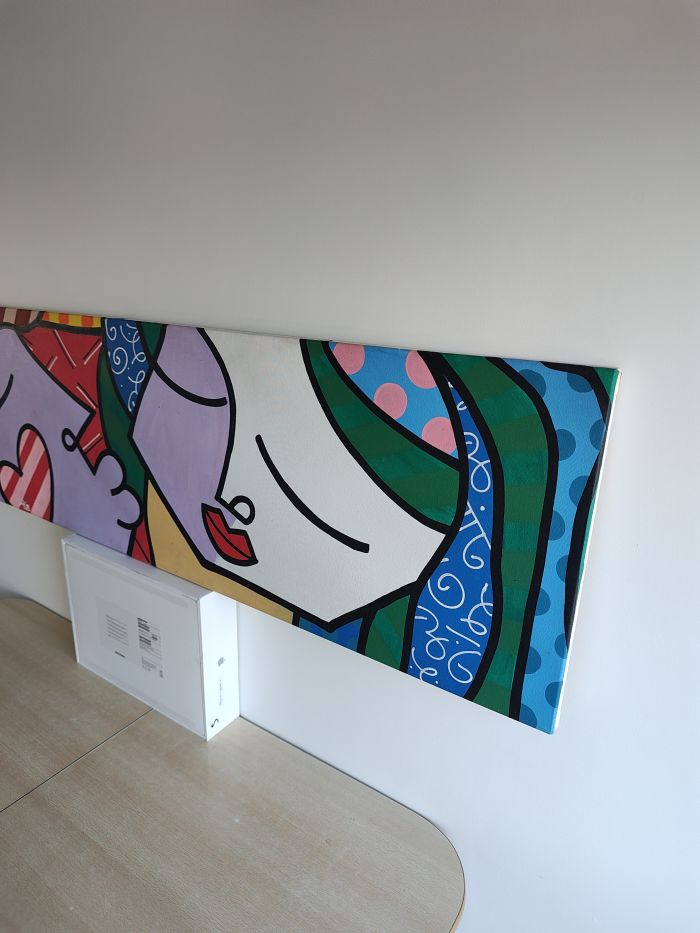
\includegraphics[width=0.32\linewidth]{cuadro_2_thumb.jpg}
\caption{Conjunto \textit{cuadro}: tres tomas con solapamiento del 30--40\% de un cuadro sobre una mesa.}
\label{fig:dataset_cuadro}
\end{figure}

\section{Método}

El pipeline implementado sigue el esquema general del enunciado: detección y descripción de características, A-NMS, matching, estimación de homografía (manual y por RANSAC), cálculo del lienzo óptimo, y stitching con blending. Todo el código se encuentra en \texttt{tp1\_panoramica/utils.py} y \texttt{tp1\_panoramica/graficos.py}, orquestado desde \texttt{Tp1\_pano.ipynb}.

\subsection{Detección y descripción de características}

Se utilizó el detector-descriptor \textbf{SIFT} (\texttt{cv2.SIFT\_create}), por su invariancia a escala, rotación e iluminación y su buen desempeño frente a los cambios de perspectiva presentes en ambos conjuntos. SIFT opera internamente en escala de grises, por lo que no fue necesaria una conversión previa.

\subsection{Supresión de No Máxima Adaptativa (A-NMS)}

Para evitar que las correspondencias se concentren en regiones muy texturadas de la imagen (p.\,ej.\ el propio cuadro) en desmedro del resto, se implementó A-NMS: para cada \textit{keypoint} $k_i$ se calcula el radio de supresión $R_i$ como la menor distancia a otro \textit{keypoint} $k_j$ con respuesta estrictamente mayor ($r_j > r_i$), y se conservan los $N$ puntos con mayor $R_i$. A diferencia del pseudocódigo del enunciado, no se restringe primero a un conjunto de máximos locales en una vecindad fija: el radio robusto se calcula directamente sobre la totalidad de los \textit{keypoints} detectados. Esta variante (equivalente a la formulación original de Brown et al.) da el mismo resultado cualitativo --puntos mejor distribuidos espacialmente-- con una implementación vectorizada más simple. La Fig.~\ref{fig:anms} compara los \textit{keypoints} crudos de SIFT con los obtenidos tras A-NMS.

\begin{figure}[htbp]
\centering
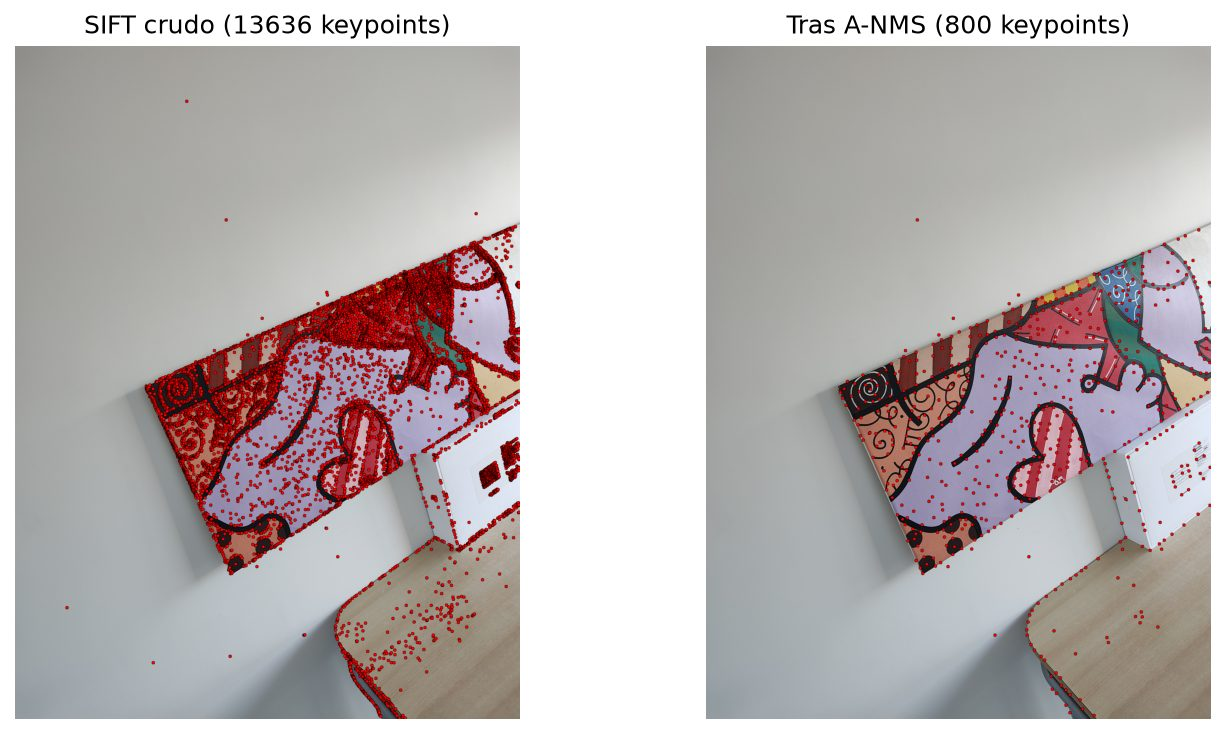
\includegraphics[width=\linewidth]{fig_anms.jpg}
\caption{Izquierda: todos los \textit{keypoints} de SIFT. Derecha: subconjunto tras A-NMS, mejor distribuido espacialmente.}
\label{fig:anms}
\end{figure}

\subsection{Asociación de correspondencias (matching)}

Se combinaron dos criterios de filtrado, aplicados en ambas direcciones (imagen 1 $\rightarrow$ 2 y 2 $\rightarrow$ 1) usando \texttt{cv2.FlannBasedMatcher} con $k=2$ vecinos:

\begin{itemize}
    \item \textbf{Test de razón de Lowe}: se descarta un match si la distancia al primer vecino no es al menos $30\%$ menor que la distancia al segundo (umbral $0.75$).
    \item \textbf{Verificación cruzada (cross-check)}: se conserva un match solo si es mutuamente el mejor en ambas direcciones.
\end{itemize}

La combinación de ambos criterios es más estricta que cualquiera por separado, lo que reduce el número final de correspondencias pero aumenta fuertemente su confiabilidad antes incluso de aplicar RANSAC (ver Sección~\ref{sec:resultados}). La Fig.~\ref{fig:matches} muestra el resultado para el par \textit{cuadro\_0-cuadro\_1}.

\begin{figure}[htbp]
\centering
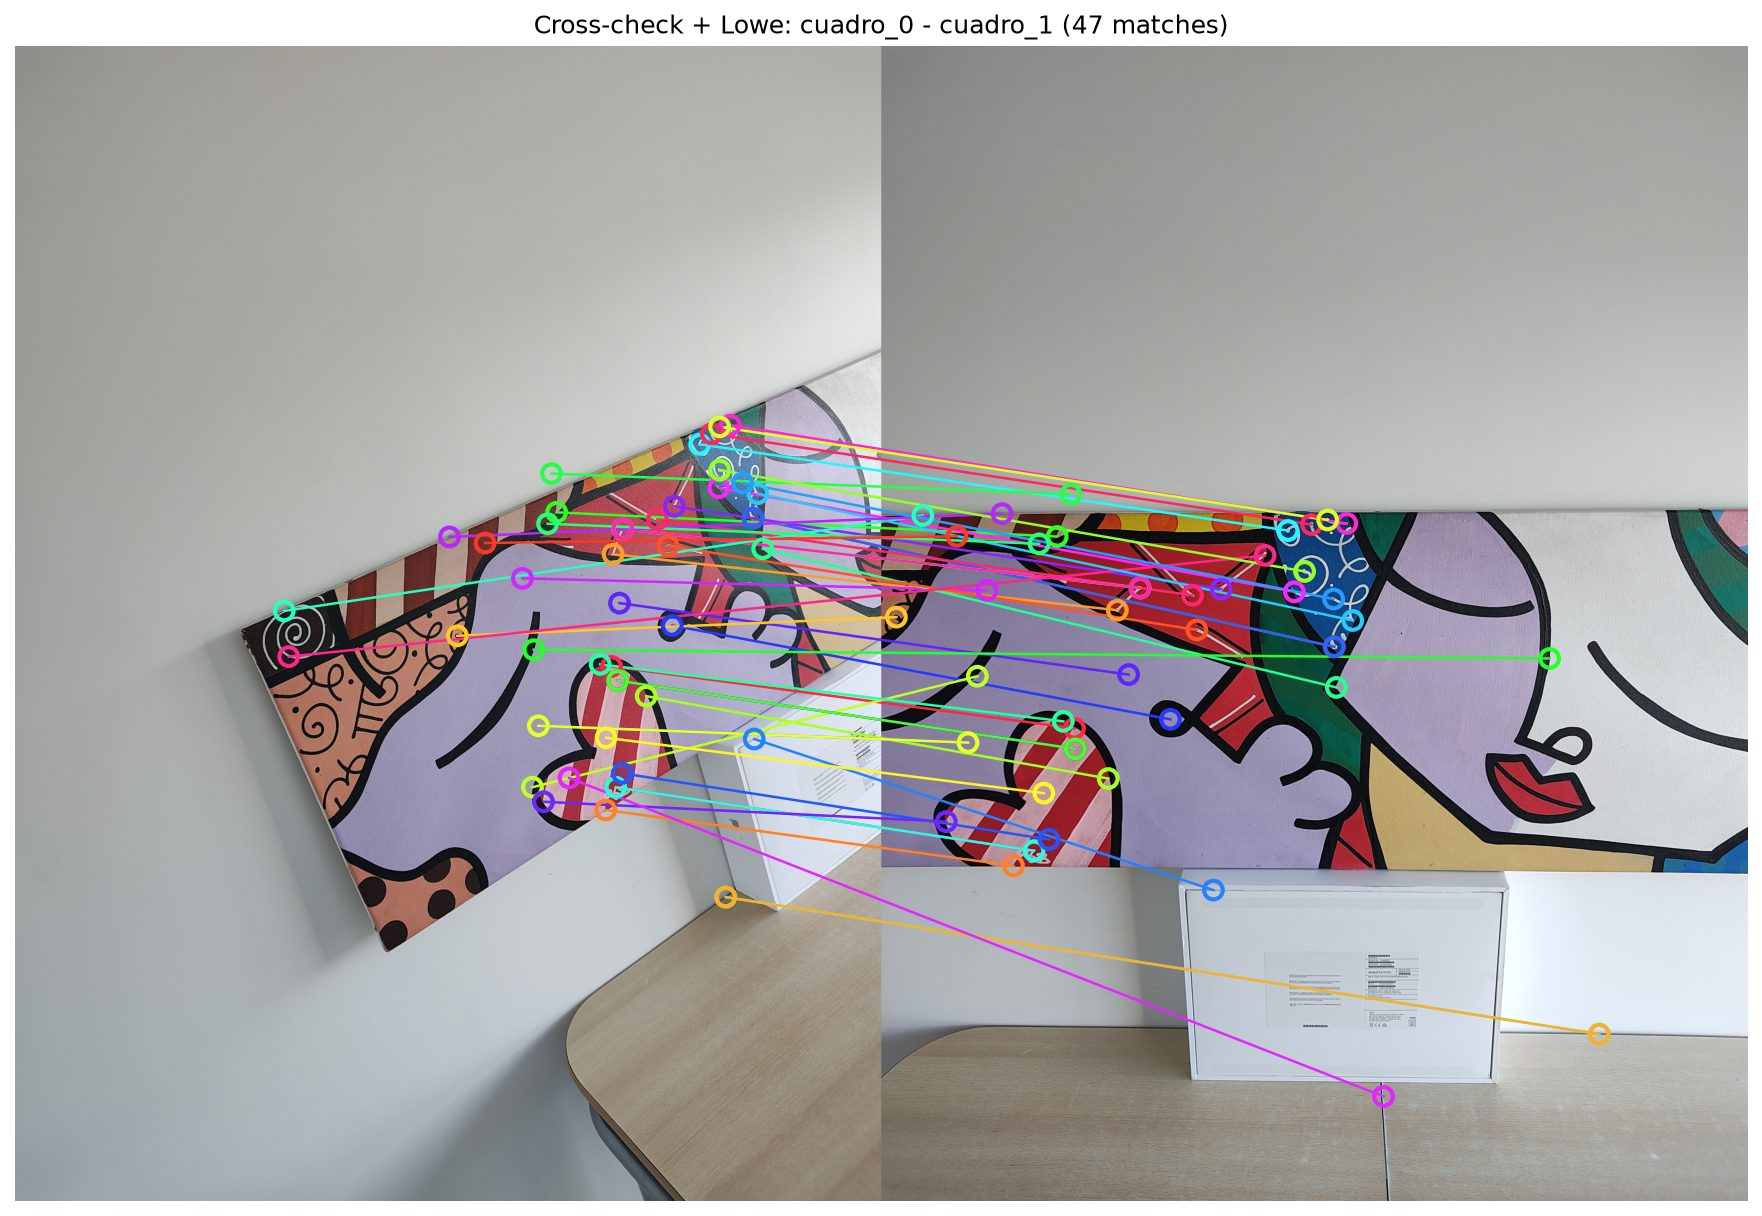
\includegraphics[width=\linewidth]{fig_matches.jpg}
\caption{Correspondencias tras cross-check + test de Lowe, cuadro\_0--cuadro\_1.}
\label{fig:matches}
\end{figure}

\subsection{Estimación manual de la homografía (DLT)}

Para uno de los pares del conjunto \textit{cuadro} se seleccionaron manualmente 4 correspondencias (Fig.~\ref{fig:dlt_puntos}), eligiendo puntos bien distribuidos espacialmente y \textbf{no colineales} (tres puntos colineales, o casi, degeneran el sistema lineal y producen una $H$ inestable o indeterminada). A partir de estos 4 pares se resolvió el algoritmo \textbf{DLT} (\textit{Direct Linear Transformation}) sin usar OpenCV: cada correspondencia $(x,y)\leftrightarrow(x',y')$ aporta dos filas a una matriz $A\in\mathbb{R}^{2N\times9}$ a partir de $\mathbf{x}'\times(H\mathbf{x})=0$, y $H$ se obtiene como el vector singular derecho asociado al menor valor singular de $A$ (SVD). Previamente se normalizan los puntos (normalización de Hartley: centrar en el origen y escalar para que la distancia media al origen sea $\sqrt{2}$) para mejorar el condicionamiento numérico del sistema. La Fig.~\ref{fig:dlt_warp} muestra el resultado de proyectar \textit{cuadro\_0} sobre \textit{cuadro\_1} con la $H$ obtenida.

\begin{figure}[htbp]
\centering
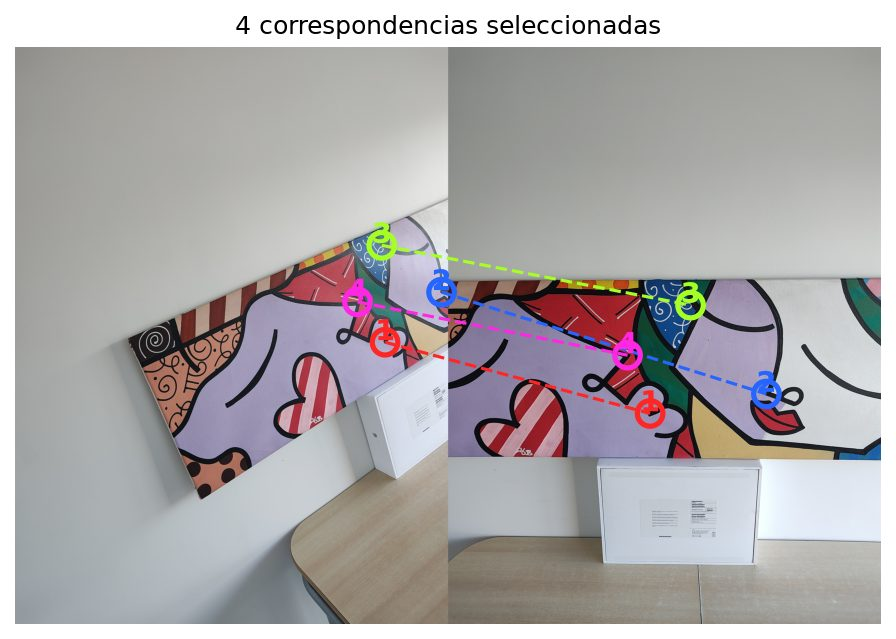
\includegraphics[width=\linewidth]{fig_dlt_puntos.jpg}
\caption{Cuatro correspondencias elegidas manualmente entre cuadro\_0 y cuadro\_1.}
\label{fig:dlt_puntos}
\end{figure}

\begin{figure}[htbp]
\centering
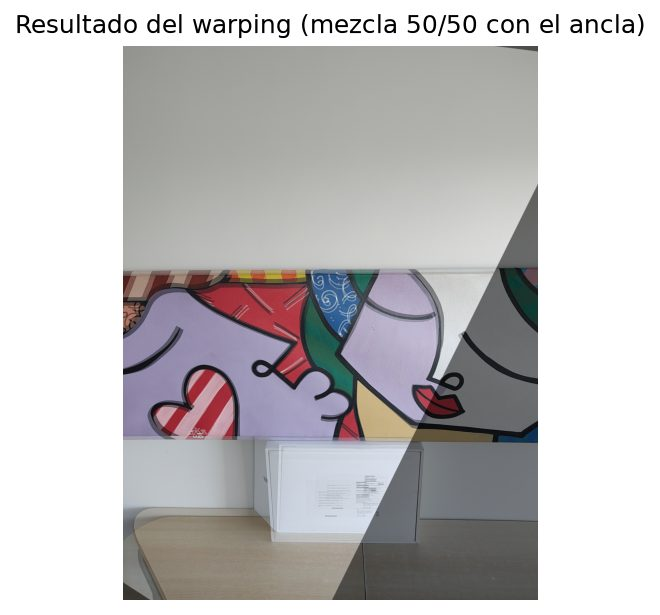
\includegraphics[width=0.85\linewidth]{fig_dlt_warp.jpg}
\caption{Mezcla 50/50 de cuadro\_1 con cuadro\_0 proyectada mediante la $H$ estimada por DLT manual.}
\label{fig:dlt_warp}
\end{figure}

\subsection{RANSAC para eliminación de outliers}

Dado que el matching automático produce correspondencias erróneas (\textit{outliers}), se implementó \textbf{RANSAC} sin OpenCV siguiendo el Algoritmo 2 del enunciado: en cada una de $T=1000$ iteraciones se muestrean 4 correspondencias al azar, se calcula $H$ con DLT, y se cuentan los \textit{inliers} --pares cuya distancia de reproyección $\lVert k_j - H\cdot k_i\rVert$ es menor a un umbral $t=5$ píxeles--. Se conserva el modelo con más \textit{inliers} a lo largo de las iteraciones, y la homografía final se recalcula por DLT usando \emph{únicamente} el conjunto de \textit{inliers} del mejor modelo (mínimos cuadrados sobreajustado, más estable que los 4 puntos mínimos). La Fig.~\ref{fig:ransac} muestra los \textit{inliers} finales para ambos pares del conjunto \textit{cuadro}.

\begin{figure}[htbp]
\centering
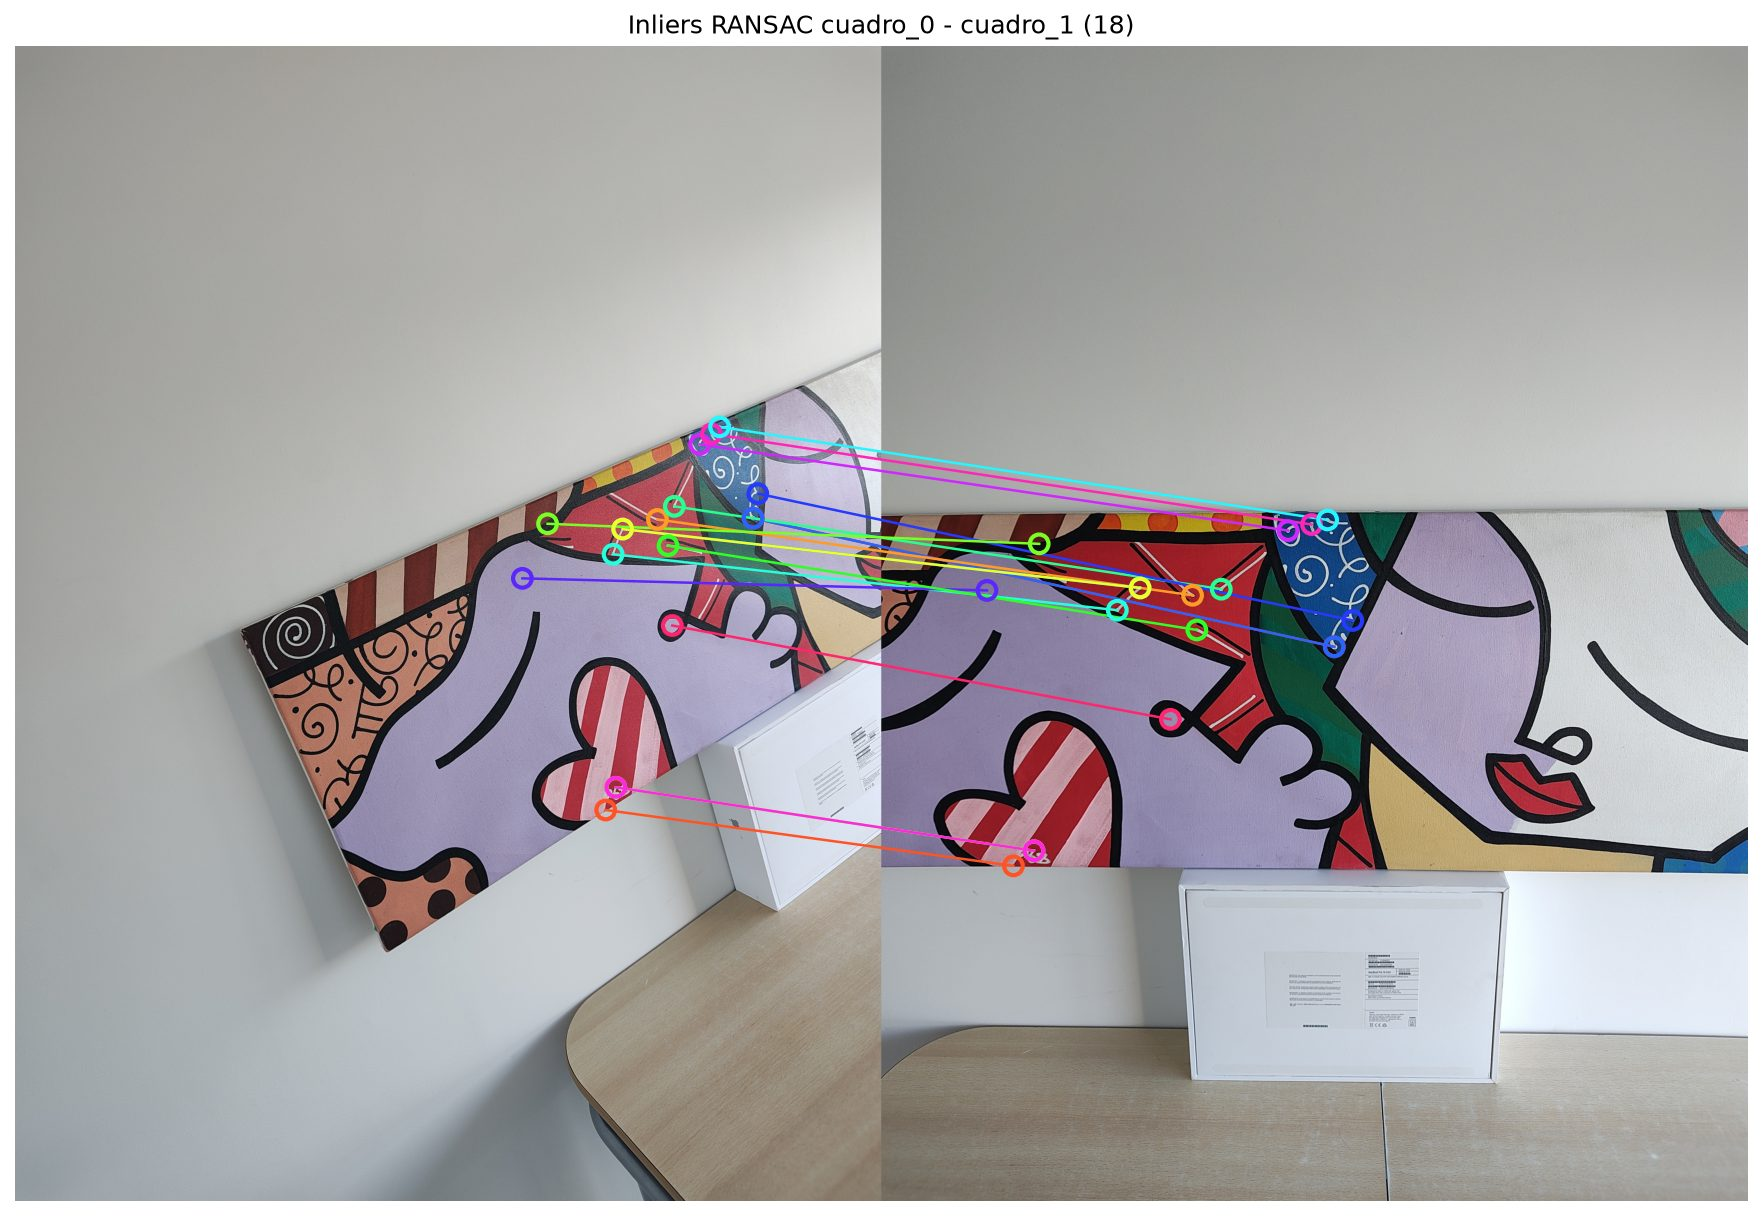
\includegraphics[width=\linewidth]{fig_ransac_01.jpg}\\
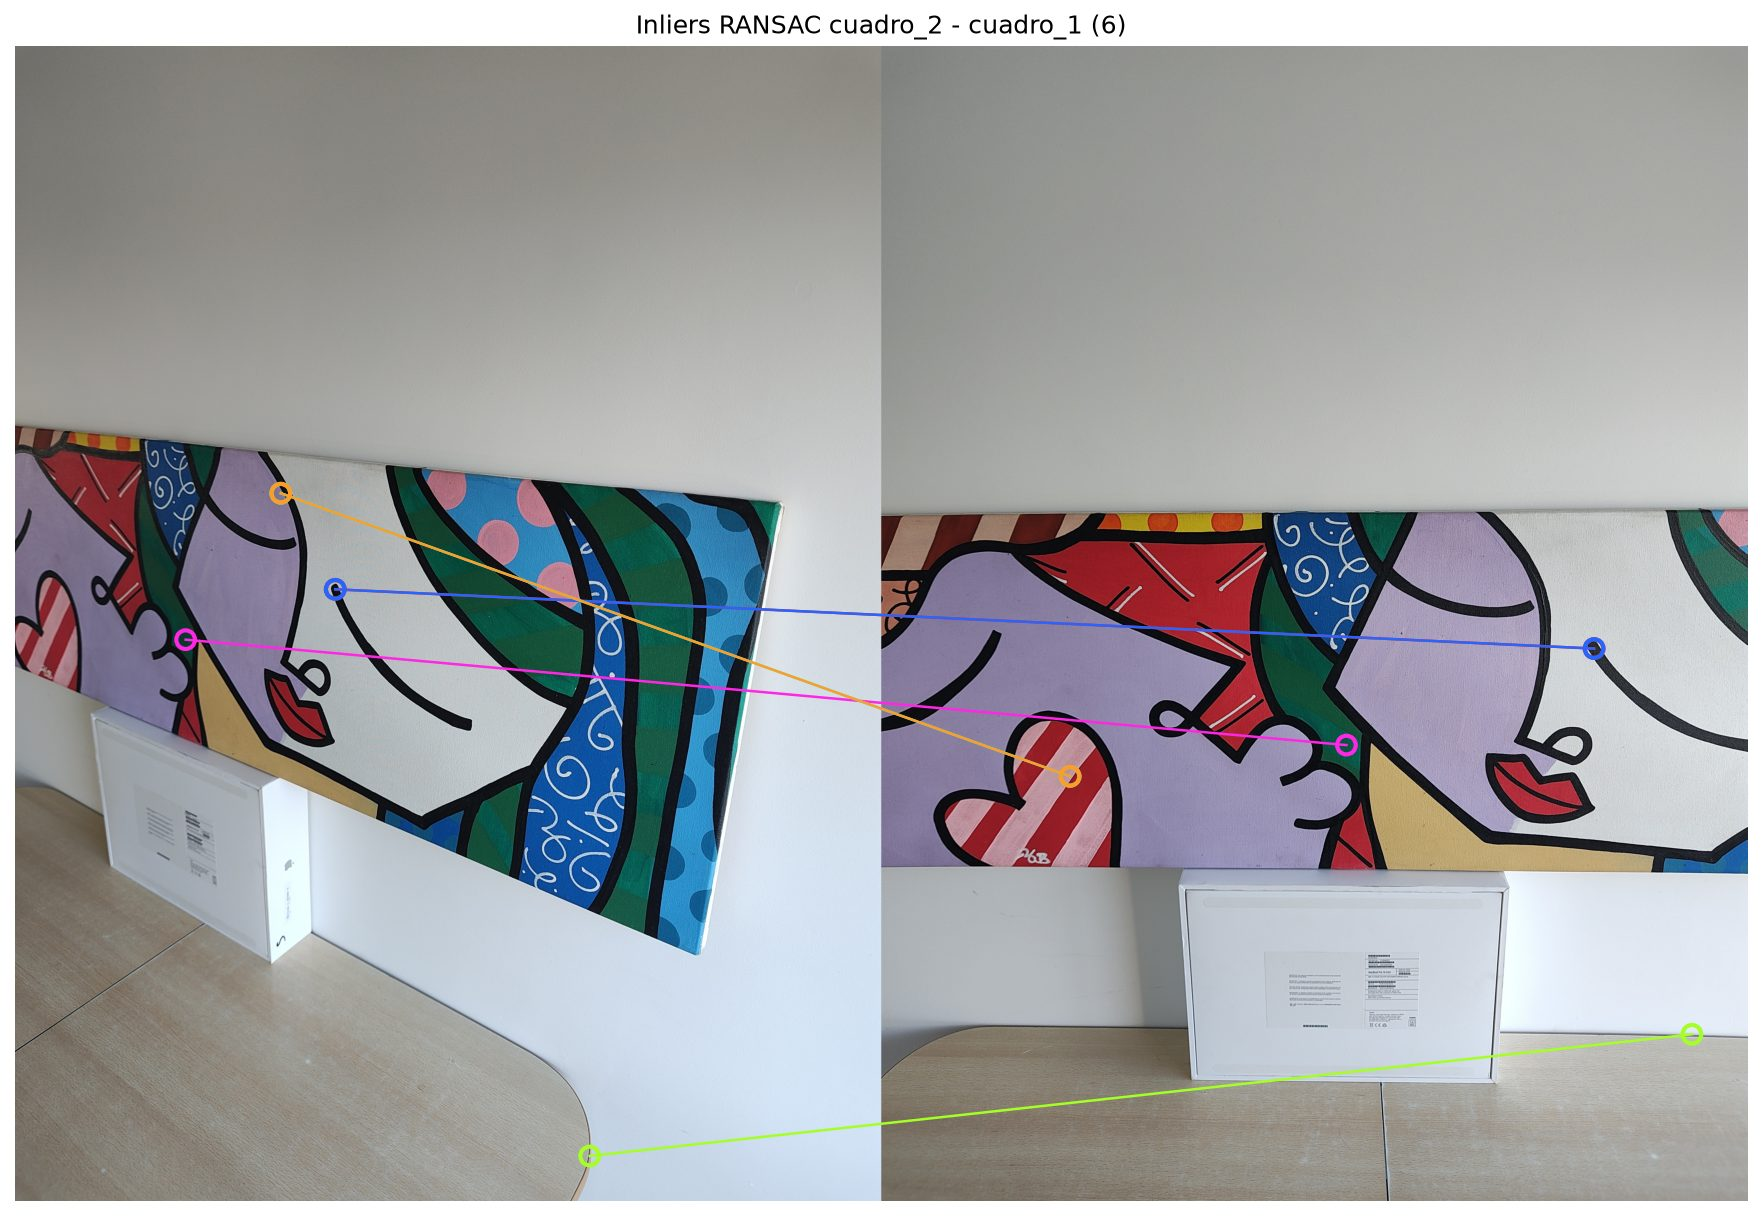
\includegraphics[width=\linewidth]{fig_ransac_21.jpg}
\caption{Correspondencias \textit{inlier} tras RANSAC. Arriba: cuadro\_0--cuadro\_1. Abajo: cuadro\_2--cuadro\_1.}
\label{fig:ransac}
\end{figure}

\subsection{Cálculo del tamaño óptimo del lienzo}

Para que la imagen final no tenga bordes negros innecesarios ni recorte contenido, se proyectan las 4 esquinas de cada imagen lateral al sistema de referencia de la imagen ancla usando su homografía ($H_{izq}$, $H_{der}$, con \texttt{cv2.perspectiveTransform}), y se agrupan junto con las esquinas de la propia imagen ancla. Tomando el mínimo y máximo de las coordenadas $x$ e $y$ de ese conjunto se obtiene el \textit{bounding box} que contiene a las tres imágenes ya proyectadas. El ancho y alto del lienzo final son, respectivamente, $x_{max}-x_{min}$ y $y_{max}-y_{min}$, y se construye una matriz de traslación pura
\[
T = \begin{pmatrix} 1 & 0 & -x_{min} \\ 0 & 1 & -y_{min} \\ 0 & 0 & 1 \end{pmatrix}
\]
que se antepone a cada homografía ($T\cdot H_{izq}$, $T$, $T\cdot H_{der}$ para la imagen ancla) antes de aplicar \texttt{cv2.warpPerspective}, de modo que todo el contenido proyectado caiga dentro de coordenadas no negativas y el lienzo tenga exactamente el tamaño necesario.

\subsection{Stitching y blending}

Cada imagen se proyecta sobre el lienzo común con \texttt{cv2.warpPerspective}. Para evitar costuras visibles se calcula, por imagen, un mapa de pesos $W_i$ mediante \texttt{cv2.distanceTransform} sobre la máscara binaria de contenido no negro: los píxeles más alejados del borde de la imagen (y por lo tanto más confiables) reciben mayor peso. El píxel final en cada canal de color se obtiene como el promedio ponderado
\[
I = \frac{\sum_i W_i \cdot I_i}{\sum_i W_i},
\]
aplicado de forma independiente e idéntica a los tres canales RGB (los pesos $W_i$ no dependen del color, por lo que el resultado es equivalente a promediar canal por canal).

\section{Resultados}
\label{sec:resultados}

\begin{table}[htbp]
\caption{Matches, inliers y error de reproyección por par de imágenes}
\begin{center}
\begin{tabular}{l c c c c}
\hline
\textbf{Par} & \textbf{Matches} & \textbf{Inliers} & \textbf{\% Inliers} & \textbf{Error (px)} \\
\hline
cuadro 0--1 & 145 & 67 & 46\% & 2.50 \\
cuadro 2--1 & 56 & 9 & 16\% & 1.43 \\
propio 0--1 & 565 & 347 & 61\% & 2.03 \\
propio 2--1 & 456 & 257 & 56\% & 0.83 \\
\hline
\end{tabular}
\label{tab:resultados}
\end{center}
\end{table}

La Tabla~\ref{tab:resultados} resume los resultados cuantitativos ($T=1000$, $t=5$ px). El error de reproyección promedio sobre los \textit{inliers} finales es de pocos píxeles en ambos pares del conjunto \textit{cuadro}, lo que indica una $H$ bien ajustada. Sin embargo, el par cuadro\_2--cuadro\_1 tiene solo 9 \textit{inliers} sobre 56 matches iniciales (16\%): esto sugiere que el solapamiento real entre esas dos tomas es menor al 30--40\% sugerido, o que la combinación estricta de cross-check + Lowe está descartando correspondencias válidas en la zona con menos textura del fondo. Aun con pocos \textit{inliers}, 9 puntos son suficientes para una $H$ estable dado el bajo error de reproyección obtenido.

El conjunto propio, con mayor cantidad absoluta de textura visual (fachada del edificio, ventanas, árboles), produjo muchas más correspondencias y una proporción de \textit{inliers} más alta y estable en ambos pares, consistente con el análisis de la Sección~I: al aproximarse mejor a una rotación pura de cámara, el modelo de homografía es más preciso en más regiones de la imagen.

\begin{figure}[htbp]
\centering
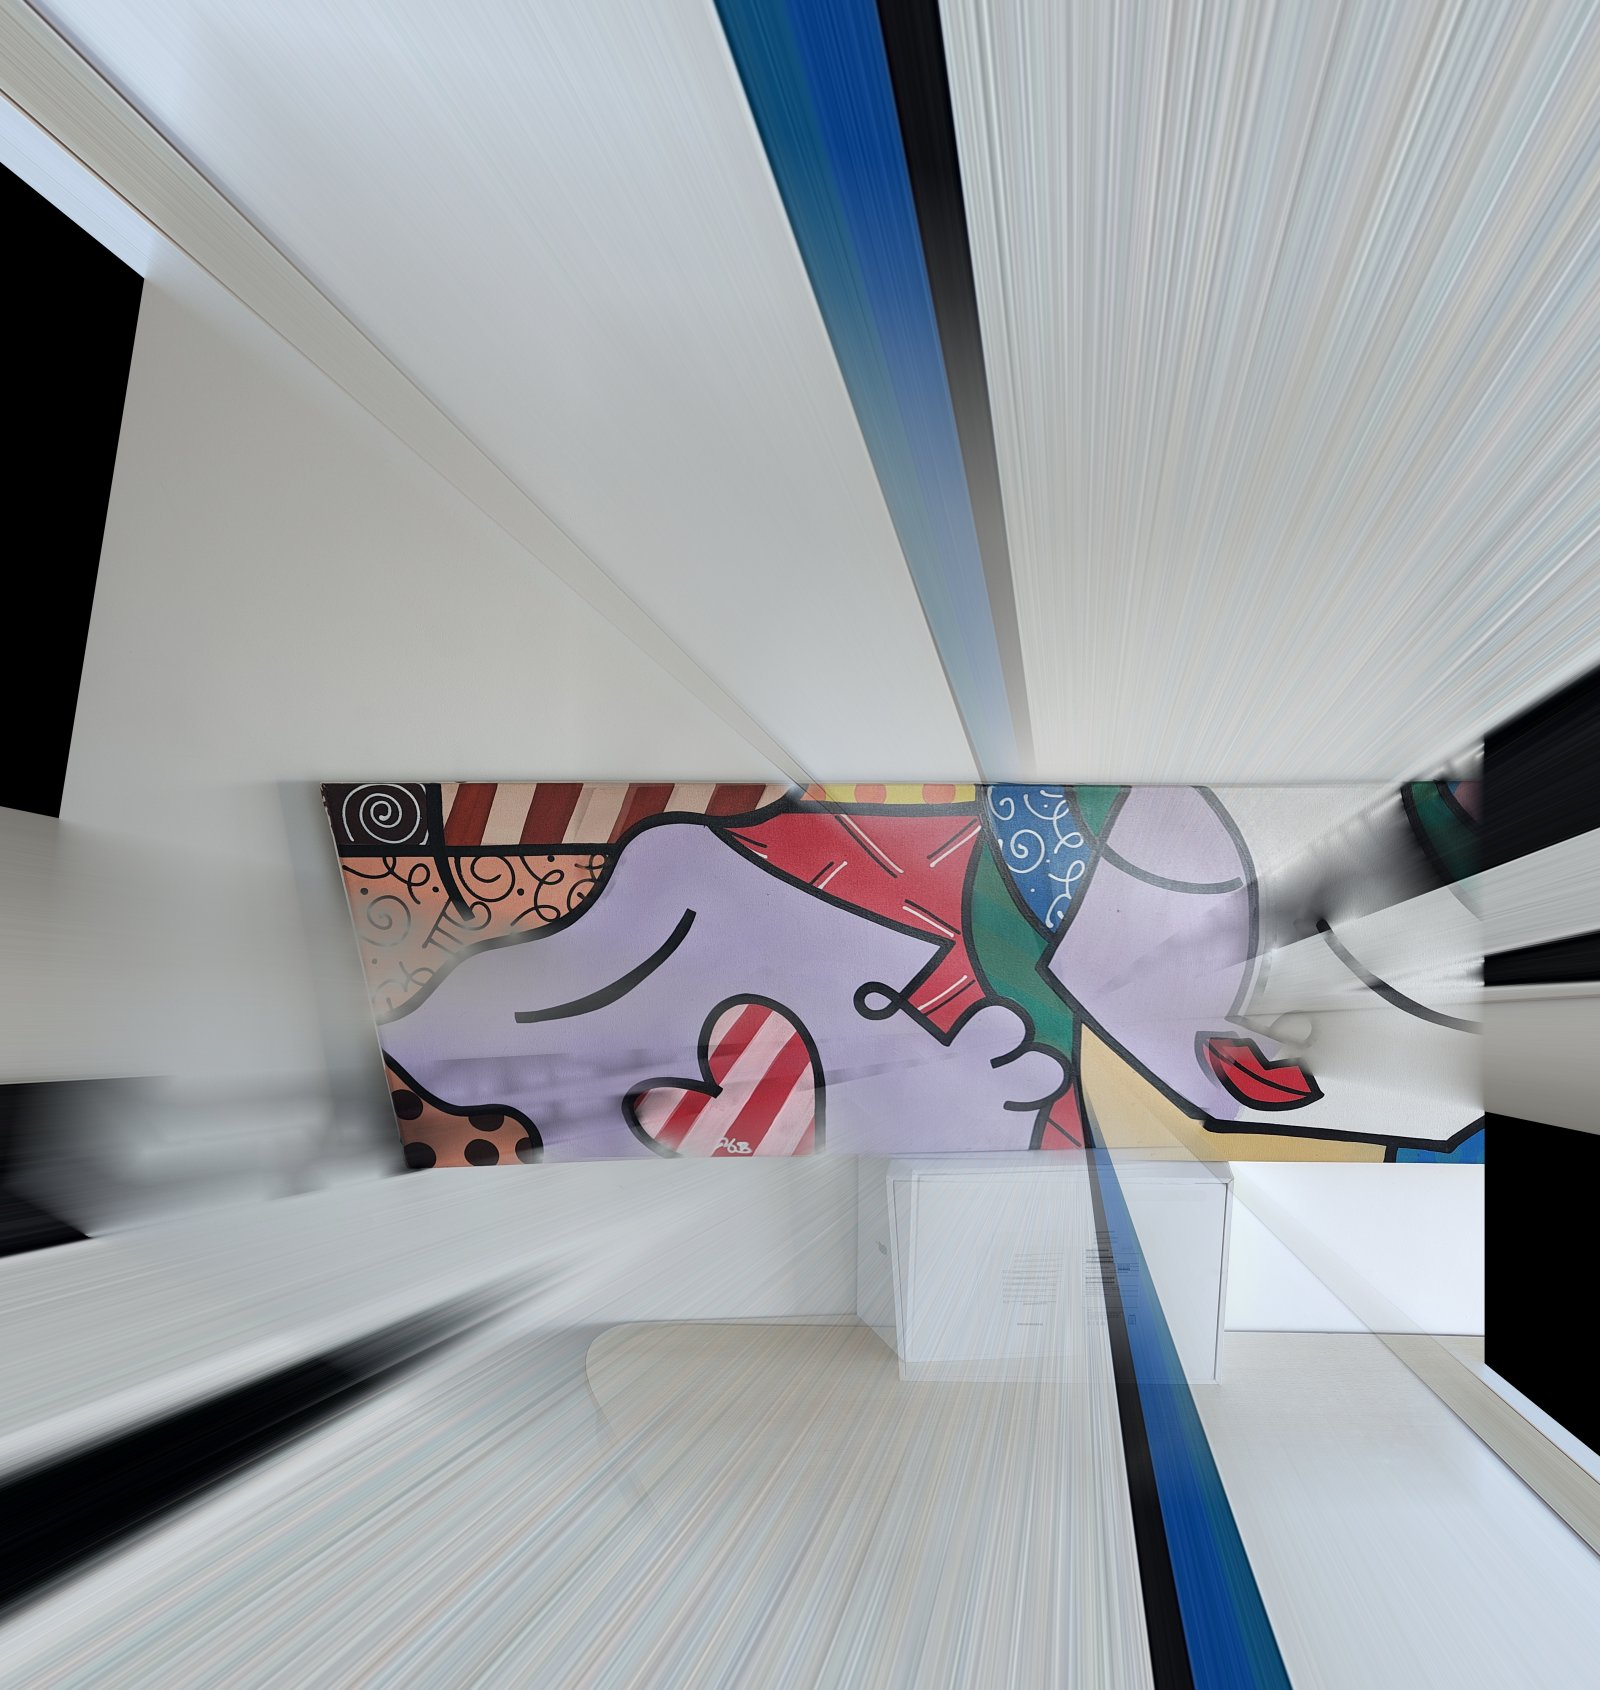
\includegraphics[width=\linewidth]{fig_panorama_cuadro.jpg}
\caption{Panorámica final del conjunto \textit{cuadro}, con blending por transformada de distancia.}
\label{fig:panorama_cuadro}
\end{figure}

\begin{figure}[htbp]
\centering
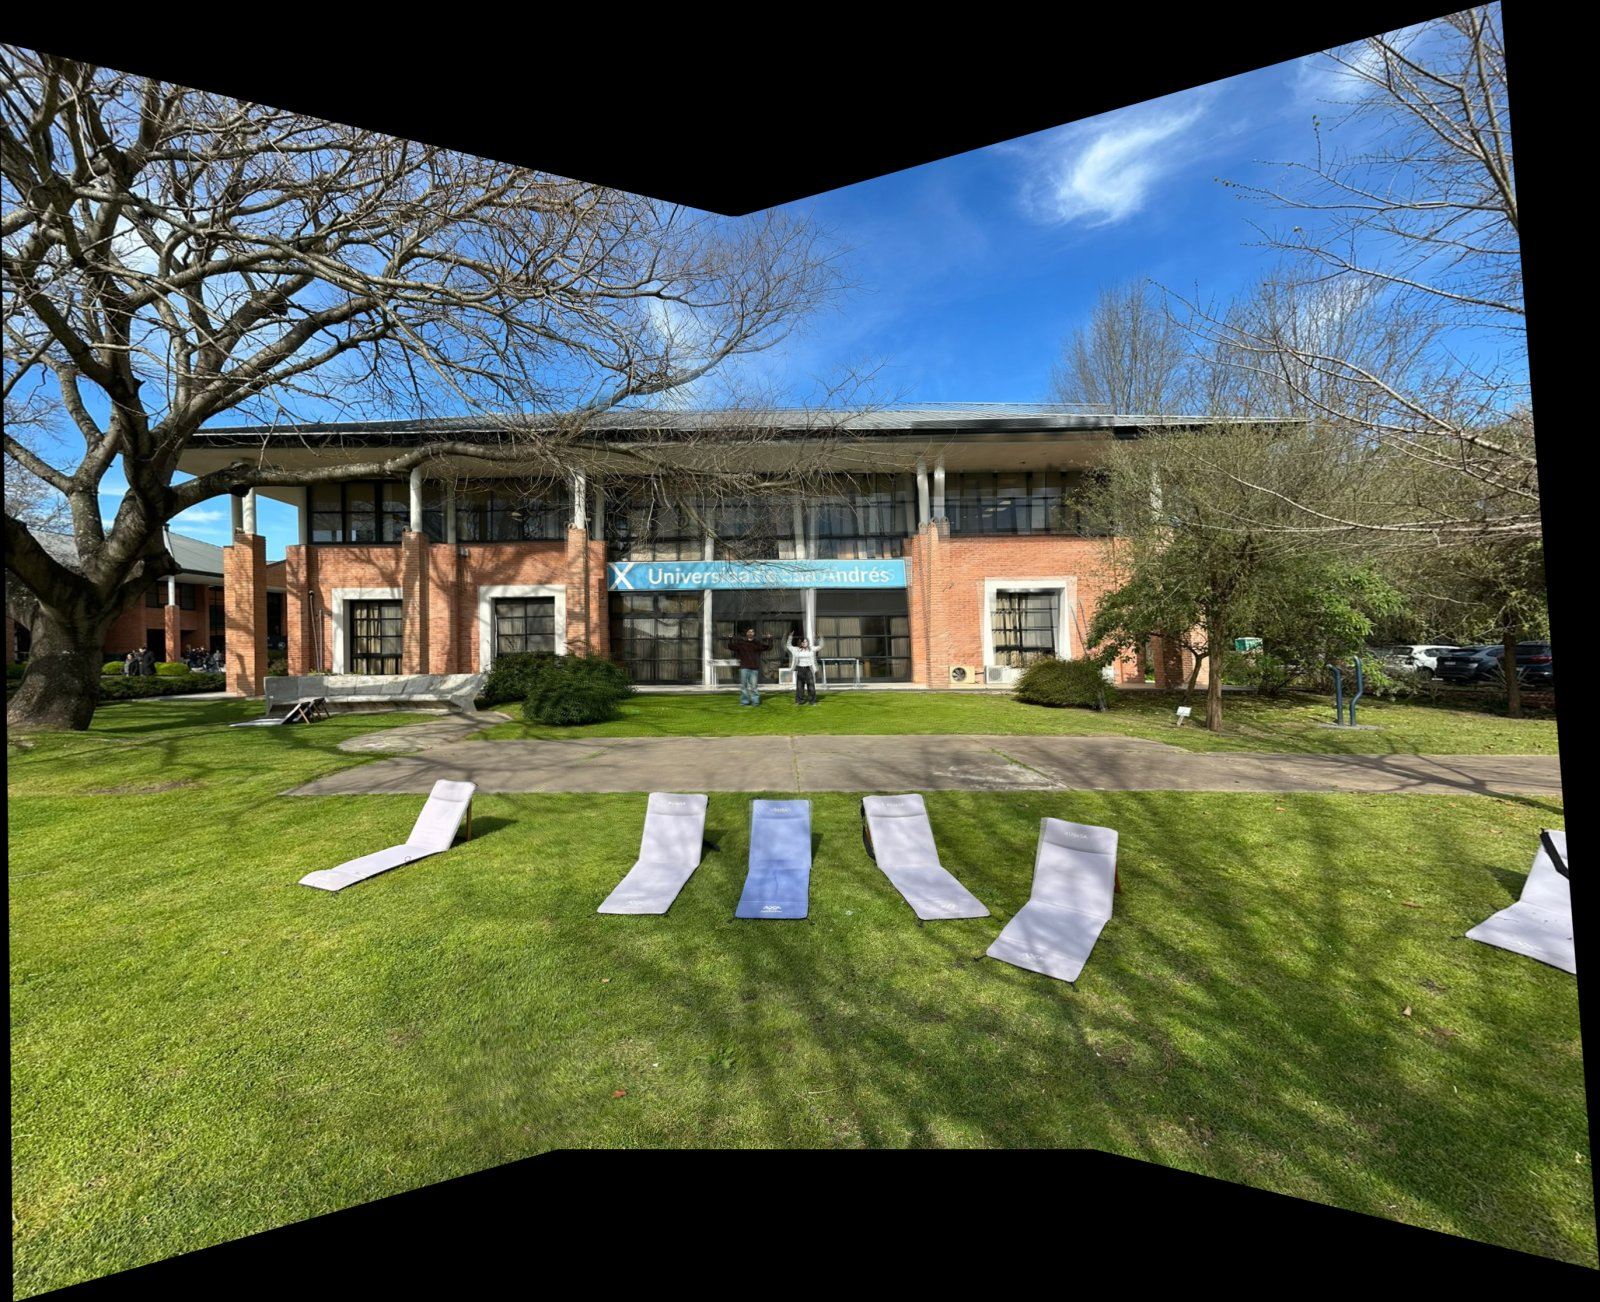
\includegraphics[width=\linewidth]{fig_panorama_foto.jpg}
\caption{Panorámica final del conjunto propio (campus de la universidad).}
\label{fig:panorama_propio}
\end{figure}

Las Fig.~\ref{fig:panorama_cuadro} y \ref{fig:panorama_propio} muestran los resultados finales. En ambos casos el lienzo tiene el tamaño óptimo (sin bordes negros sobrantes ni recorte de contenido) y la transición entre imágenes es suave gracias al blending por distancia. En el conjunto propio se observa un leve \textit{ghosting} en los árboles más cercanos a la cámara, consistente con el paralaje residual discutido en la introducción.

\section{Conclusiones}

Se implementó un pipeline completo de \textit{stitching} panorámico --detección SIFT, A-NMS, matching con cross-check y test de Lowe, DLT manual, RANSAC, cálculo de lienzo óptimo y blending por distancia-- validado sobre un conjunto provisto y uno propio, con errores de reproyección finales de pocos píxeles. Como trabajo futuro, el número de iteraciones de RANSAC podría adaptarse dinámicamente según la proporción estimada de \textit{inliers} en lugar de fijarse en $T=1000$, y el pipeline de blending --actualmente escrito específicamente para 3 imágenes (izquierda-centro-derecha)-- podría generalizarse a $N$ imágenes arbitrarias.

\begin{thebibliography}{00}
\bibitem{lowe2004} D. G. Lowe, ``Distinctive Image Features from Scale-Invariant Keypoints,'' \textit{International Journal of Computer Vision}, vol. 60, no. 2, pp. 91--110, 2004.
\bibitem{brown2005} M. Brown, R. Szeliski, and S. Winder, ``Multi-Image Matching using Multi-Scale Oriented Patches,'' in \textit{Proc. IEEE CVPR}, 2005.
\bibitem{hartley1997} R. I. Hartley, ``In Defense of the Eight-Point Algorithm,'' \textit{IEEE Trans. Pattern Analysis and Machine Intelligence}, vol. 19, no. 6, pp. 580--593, 1997.
\bibitem{fischler1981} M. A. Fischler and R. C. Bolles, ``Random Sample Consensus: A Paradigm for Model Fitting with Applications to Image Analysis and Automated Cartography,'' \textit{Communications of the ACM}, vol. 24, no. 6, pp. 381--395, 1981.
\bibitem{szeliski2006} R. Szeliski, ``Image Alignment and Stitching: A Tutorial,'' \textit{Foundations and Trends in Computer Graphics and Vision}, vol. 2, no. 1, pp. 1--104, 2006.
\end{thebibliography}

\end{document}
